\documentclass[12pt, a4paper]{article}
\usepackage[a4paper, includeheadfoot, mag=1000, left=2cm, right=1.5cm, top=1.5cm, bottom=1.5cm, headsep=0.8cm, footskip=0.8cm]{geometry}
% Fonts
\usepackage{fontspec, unicode-math}
\setmainfont[Ligatures=TeX]{CMU Serif}
\setmonofont{CMU Typewriter Text}
\usepackage[english, russian]{babel}
% Indent first paragraph
\usepackage{indentfirst}
\setlength{\parskip}{5pt}
% Page headings
\usepackage{fancyhdr}
\pagestyle{fancy}
\renewcommand{\headrulewidth}{0pt}
\setlength{\headheight}{16pt}
\newfontfamily\namefont[Scale=1.2]{Gloria Hallelujah}
\fancyhead{}
% Use case template
\newcommand{\uctitle}[1]{\renewcommand{\givenuctitle}{#1}}
\newcommand{\givenuctitle}{Не указано}
\newcommand{\ucgoal}[1]{\renewcommand{\givenucgoal}{#1}}
\newcommand{\givenucgoal}{Не указано}
\newcommand{\ucscenario}[1]{\renewcommand{\givenucscenario}{#1}}
\newcommand{\givenucscenario}{\item Не указано}
\newcommand{\ucextensions}[1]{\renewcommand{\givenucextensions}{#1}}
\newcommand{\givenucextensions}{\item Не указано}
\newenvironment{usecase}{}{
  \noindent\fbox{
    \parbox{0.98\textwidth}{
      \vspace{2mm}
      \textbf{\large \givenuctitle}\\[3mm]
      \textbf{Цель:} \givenucgoal\\[2mm]
      \textbf{Сценарий:}
      \begin{enumerate}\givenucscenario\end{enumerate}
      \textbf{Расширения:}
      \begin{itemize}\givenucextensions\end{itemize}
    }
  }
}

\begin{document}

% Title page
\begin{titlepage}
\begin{center}

\textsc{ФГАОУ ВО «Санкт-Петербургский национальный исследовательский университет информационных технологий, механики и оптики»\\[4mm]
Кафедра вычислительной техники}
\vfill
\textbf{КУРСОВАЯ РАБОТА\\[4mm]
Программирование интернет-приложений}\\[16mm]
Саржевский Иван Анатольевич
\\[2mm]Лабушев Тимофей Михайлович
\\[2mm]Группа P3202
\vfill
Санкт-Петербург\\[2mm]
2018 г.

\end{center}
\end{titlepage}


% Table of contents
\begin{center}
{\namefont\huge Sumaju nikki}\\[6mm]
\textsc{Браузерная многопользовательская текстовая игра\\
жанра Zero-Player Game}
\vspace{4mm}
\end{center}
\tableofcontents
\newpage

% Contents
\fancyhead[R]{\namefont Sumaju nikki}

\section{Введение}

Предметом разработки является платформа для многопользовательской текстовой игры
жанра \textit{Zero-Player Game (ZPG)}, использующая браузерный интерфейс и
сохраняющая прогресс игрока на игровом сервере.

В основе жанра лежит концепция протекания игрового процесса
без вмешательства со стороны пользователя. При этом игроку предоставляются
возможности ускорения своего игрового прогресса и
взаимодействия с другими пользователями.

Предполагается, что взаимодействие с платформой будет представлять собой
не длинные сессии, свойственные традиционным играм, а короткие, но частые
посещения, характерные для социальных сетей.

\subsection{Цель создания}

Платформа разрабатывается с целью предоставления творческим молодым людям
возможности самовыражения в игровой форме. Платформа предоставляет набор
базовых игровых механик, в то время как содержательная часть создается
самими пользователями, путём предоставления возможности формировать
предложения для контента

\subsection{Целевая аудитория}

Творческие молодые люди, в возрасте 18-25 лет, знакомые с современными медиа,
активные пользователи интернета. Не имеют времени/желания проводить много
времени за игрой в компьютерные игры, ищут более подходящего под свой стиль
жизни формата.


\section{Прецеденты использования}

\begin{usecase}
\uctitle{Регистрация}
\ucgoal{Завести аккаунт в cистеме, создать персонажа}
\ucscenario{
  \item Незарегестрированный пользователь открывает любую страницу платформы.
  \item Система перенаправляет пользователя на главную страницу с формой регистрации.
  \item Пользователь вводит адрес электронной почты и пароль, отправляет форму.
  \item Система создает аккаунт и перенаправляет пользователя на страницу
    создания персонажа.
  \item Пользователь указывает имя и пол персонажа, опционально загружает картинку,
    отправляет форму.
  \item Система авторизует пользователя.
}
\ucextensions{
  \item На шаге 3 пользователю предоставляется возможность регистрации используя
    аккаунт социальной сети.
  \item Ошибка на шаге 4 (адрес электронной почты уже используется, пароль содержит
    менее восьми символов) предотвращает переход к следущему шагу.
}
\end{usecase}

\begin{usecase}
\uctitle{Авторизация}
\ucgoal{Войти в систему}
\ucscenario{
  \item Незарегестрированный пользователь открывает любую страницу платформы.
  \item Система перенаправляет пользователя на главную страницу с формой входа.
  \item Пользователь вводит адрес электронной почты и пароль, отправляет форму.
  \item Система авторизует пользователя и перенаправляет его на страницу персонажа.
}
\ucextensions{
  \item На шаге 3 пользователю предоставляется возможность авторизоваться, используя
    аккаунт социальной сети.
  \item На шаге 4 возникновение ошибки (адрес электронной почты уже используется,
    пароль содержит менее восьми символов) предотвращает переход к следущему шагу.
}
\end{usecase}

\begin{usecase}
\uctitle{Наблюдение за игровым процессом}
\ucgoal{Отследить развитие персонажа, прочесть интересные записи в дневнике}
\ucscenario{
  \item Авторизованный пользователь открывает страницу персонажа.
  \item Система предоставляет обзор характеристик персонажа, его текущее занятие и
    цели для повышения уровня.
  \item За один клик пользователь имеет возможность перейти к дневнику персонажа,
    энциклопедии известных персонажу существ, карте мира.
}
\ucextensions{
  \item Пользователь может увидеть краткую информацию о состоянии персонажа
    (его здоровье и текущее занятие) в шапке любой страницы игрового портала.
}
\end{usecase}

\begin{usecase}
\uctitle{Участие в игровом процессе}
\ucgoal{Оказать влияние на развитие персонажа}
\ucscenario{
  \item Авторизованный пользователь открывает меню \textit{сов} с помощью кнопки,
    доступной в шапке любой страницы игрового портала.
  \item Пользователь выбирает из списка доступных сов одну.
  \item Система добавляет сову во внутреннюю очередь эффектов хода, уменьшает
    количество доступных сов выбранного типа на одну, показывает пользователю
    уведомление об успешном начале полета птицы.
  \item По завершению хода в дневнике персонажа появляется заметка о действии совы.
}
\ucextensions{
  \item Число возможных сов одного типа ограничено, что должно быть понятно
    пользователю из интерфейса системы.
}
\end{usecase}

\begin{usecase}
\uctitle{Взаимодействие с другими игроками}
\ucgoal{Повлиять на отношения персонажа с другими учениками,
  усилив таким образом влияние на персонажа сов}
\ucscenario{
  \item Авторизованный пользователь выбирает \textit{чернильную сову} из списка доступных.
  \item Система предоставляет пользователю форму с поиском персонажа-получателя по имени,
    в которой доступно автодополнение и список последних адресатов.
  \item Пользователь выбирает получателя.
  \item Система случайно выбирает \textit{клуб}, для которого создается запись о
    письме. При посещении персонажем-получателем клуба, его отношения с
    персонажем пользователя изменяются.
  \item В дневники обоих персонажей добавляется запись об изменении отношений.
}
\ucextensions{
  \item Действие невозможно, если у пользователя отсутсвует необходимый тип совы.
}
\end{usecase}

\section{Требования к аппаратно-программному обеспечению}

\subsection{Требования к серверному обеспечению}

Система, которая обеспечивает выполнение программных продуктов сервера приложений
и хранение данных платформы, должна отвечать следующим требованиям:

\begin{itemize}
\item Поддержка операционной системой бинарного интерфейса приложений (ABI) Linux
\item Наличие сервера баз данных PostgreSQL версии 9.6 и выше
\end{itemize}

\subsection{Требования к клиентскому обеспечению}

Браузерный интерфейс разрабатывается с учетом следующих требований к
программному обеспечению на стороне пользователя:

\begin{itemize}
\item веб-браузер Google Chrome версии 67 и выше или
Mozilla Firefox версии 61 и выше c включенным интерпретатором сценариев JavaScript,
\item отсутствие запрета веб-страницам платформы доступа к внешним ресурсам,
а именно изображениям, шрифтам, таблицам стилей CSS и сценариям JavaScript,
в том числе блокировщиками рекламы.
\end{itemize}

\section{Требования к архитектуре системы}

\subsection{Глоссарий}

\textbf{Уровень back-end} — серверное приложение, с которым взаимодействует
пользовательский интерфейс игры. Уровень back-end обеспечивает хранение данных,
расчет игровых процессов, взаимодействие между пользователями.

\textbf{Уровень front-end} — браузерное приложение, которое реализует
пользовательский интерфейс игры. Уровень front-end включает в себя
HTML-страницы, сценарии JavaScript, таблицы стилей CSS.

\subsection{Уровень back-end}

\begin{enumerate}
\item Серверное приложение должно разрабатываться на платформе \textit{JVM}
с использованием фреймворков \textit{Akka} и \textit{Play}.
\item Взаимодействие между уровнями front-end и back-end должно осуществляться
посредством REST API; возможно использование протокола WebSockets для реализации
обновлений в режиме реального времени.
\item Серверное приложение должно реализовывать аутентификацию пользователей
с поддержкой входа через социальные сети (OAuth), используя библиотеку
\textit{play-silhouette}. Пароли пользователей должны храниться как
криптографический хэш.
\item Серверное приложение должно публиковать push-уведомления об игровых событиях,
используя сервис \textit{Firebase Cloud Messaging}.
\item Серверное приложение должно отправлять пользователям еженедельное новостноe
сообщение электронной почты, используя \textit{JavaMail API}.
\item Серверное приложение должно предоставлять API для доступа к очереди
пользовательских предложений, а также их принятию, отклонению и редактированию
(см. раздел \ref{telegram-bot}).
\end{enumerate}

\subsection{Уровень front-end}

\begin{enumerate}
\item Клиентское приложение должно разрабатываться с использованием фреймворка Vue.js.
\item Веб-интерфейс должен быть адаптирован для отображения в трех режимах:
\textit{десктопном} (ширина экрана больше 1107px),
\textit{планшетном} (больше 889px) и \textit{мобильном} (меньше 889px).
\item Веб-интерфейс должен предоставлять пользователю возможность подписаться на
push-уведомления.
\item Веб-интерфейс должен распознаваться в мобильной ОС Android как
приложение, используя \textit{Web App Manifest}.
\end{enumerate}

\subsection{Telegram-бот}
\label{telegram-bot}

Модерация добавляемого пользователями контента должна осуществляться
при помощи Telegram-бота.

\begin{enumerate}
\item Бот должен работать в заранее определенном чате, в котором находятся администраторы платформы.
\item Предложения должны выноситься ботом по одному на обсуждение в чат. Администраторы должны иметь возможность принятия, отклонения, редактирования предложения. 
\end{enumerate}

\section{Архитектура системы}

\begin{center}
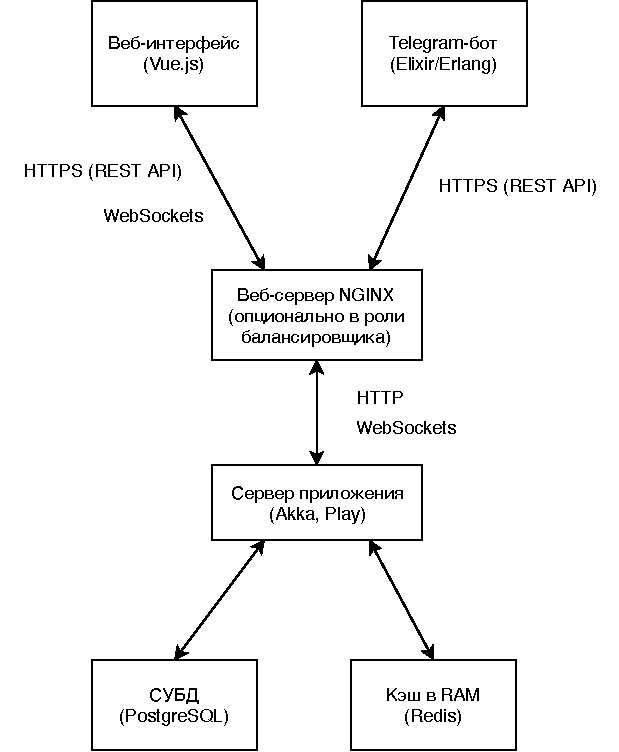
\includegraphics{architecture-overview.pdf}
\end{center}
\end{document}
